\begin{surferIntroPage}{أشكال قياسية عالمية}{record_chmutovoktic}{أشكال قياسية عالمية}

    يُقال عن منحني أنه \emph{غير متفرد} أو \emph{أملس } إذا لم يكن له رؤوس (\emph{هذه النقاط تٌسمى متفردات}). بين المنحنيات الملساء نجد الكرة و الحلقة، كما نرى في أول صورتين أدناه. بشكل عام، المنحنيات التي يتم اختيارها عشوائياً تكون ملساء.
 \begin{center}
      \vspace{-0.2cm}
      \begin{tabular}{@{}c@{}c@{}c@{\quad}c@{}c@{}c@{}c@{}}
        \begin{tabular}{@{}c@{}}
          ملساء:
        \end{tabular}
        &
        \begin{tabular}{@{}c@{}}
          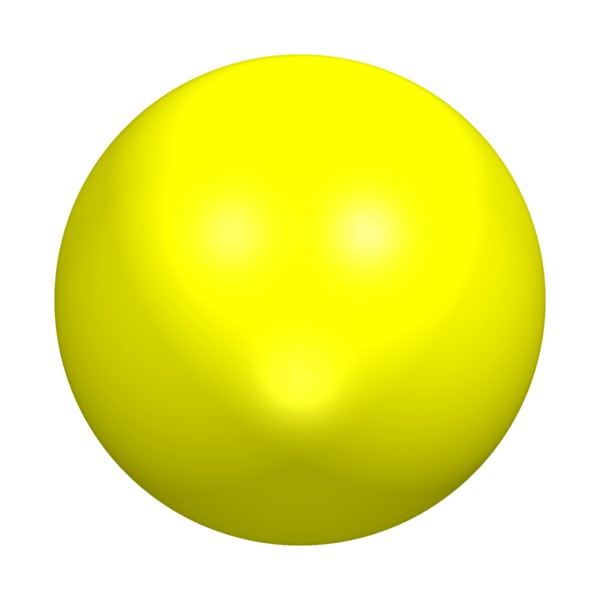
\includegraphics[width=1.1cm]{./../../common/images/kugel}
        \end{tabular}
        &
        \begin{tabular}{@{}c@{}}
          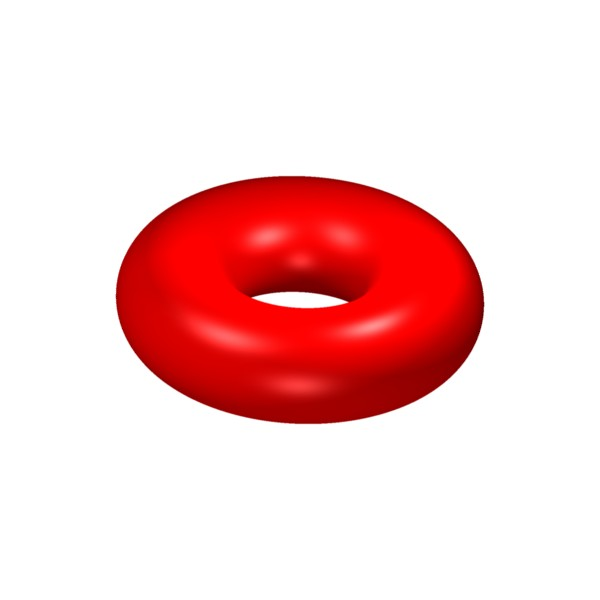
\includegraphics[width=1.1cm]{./../../common/images/torus}
        \end{tabular}
        &
        \begin{tabular}{@{}c@{}}
          عدة\\
          متفردات:
        \end{tabular}
        &
        \begin{tabular}{c@{}@{}}
          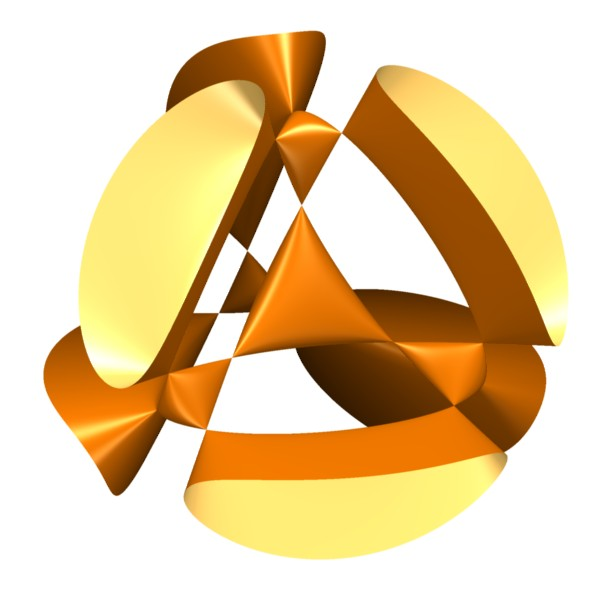
\includegraphics[width=1.1cm]{./../../common/images/kummer}
        \end{tabular}
        &
        \begin{tabular}{c@{}@{}}
          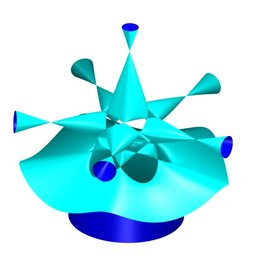
\includegraphics[width=1.1cm]{./../../common/images/togliatti}
        \end{tabular}
        &
        \begin{tabular}{c@{}@{}}
          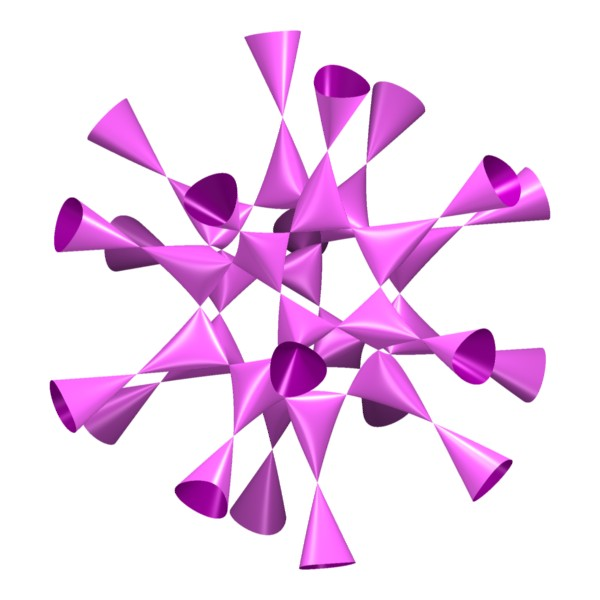
\includegraphics[width=1.1cm]{./../../common/images/barth_sextic}
        \end{tabular}
      \end{tabular}
    \end{center}
    \vspace{-0.2cm}
       ولذلك فإن المنحنيات التي تبين متفردات هي حالات خاصة للغاية. لأن المتفردات هي أكثر نقاط المنحنى جديرة بالإهتمام. تم تحديد المنحنيات في برنامج SURFER بواسطة جذور متعددات الحدود حيث تكون اسات المتغيرات أعداداً صحيحة إيجابية. أعلى قيمة حاصل جمع أسات كل أحادية حدود التي تشكل متعدد الحدود هي درجة متعدد الحدود $d$. في الرياضيات، يحاولون معرفة عدد متفردات لمنحنى له درجة معينة.
       سنشير إلى هذا العدد بواسطة $\mu(d)$.

لقد تبين أنه من الصعب جداً حساب هذا العدد $\mu(d)$.
قيمة $\mu(d)$ معروفة منذ القرن التاسع عشر لكل من $d=1,2,3,4$، ولكن في حال $d=5$، لم يتم تحديد هذا العدد حتى العام 1980، وفي حال $d=6$، في العام 1996.
   في حال $d\ge 7$، لا يزال العدد $\mu(d)$ غير معروف.


    كل رقم قياسي عالمي جديد يأخذه $\mu(d)$  يشكل نتيجة جزئية مهمة. يبدو أنه يلزم وقت أطول بكثير لحل هذه المسألة مع درجة $d$ عشوائية.\\ بعض النتائج المعروفة:

   \begin{center}
      \begin{tabular}{r|cccccccc|c}
        $d$ & $1$ & $2$ & $3$ & $4$ & $5$ & $6$ & $7$ & $8$ & $d$\\
        \hline
        \hline
        \rule{0pt}{1.2em}$\mu(d)\ge$ & $0$ & $1$ & $4$ & $16$ & $31$ & $65$ &
        $99$ & $168$ &
        $\approx \frac{5}{12}d^3$\\[0.3em]
        \hline
        \rule{0pt}{1.2em}$\mu(d)\le$ & $0$ & $1$ & $4$ & $16$ & $31$ & $65$ &
        $104$ & $174$ & $\approx \frac{4}{9}d^3$
      \end{tabular}
    \end{center}
\end{surferIntroPage}
